\section{Il modello di coalescenza}
Nel modello di coalescenza, i nucleoni generati dalla collisione vanno a formare un nucleo se essi sono vicini nello spazio delle fasi.
Per comprendere meglio, il modello si incentra su un parametro $B_A$, detto \emph{di coalescenza}, il quale è un indicatore della probabilità di formazione del nucleo.
Esso è definito nel seguente modo \cite{alice_2022_coal_formula}:
\begin{equation}\label{eq:coal}
    \dfrac{1}{2\pi p_t^\text{A}}\dfrac{d^2N_\text{A}}{dy\ dp_t^\text{A}} = B_\text{A}({p_t}^\text{p}) \cdot  \left(\dfrac{1}{2\pi p_t^\text{p}}\dfrac{d^2N_\text{p}}{dy\ dp_t^\text{p}}\right)^A
\end{equation}
con p e A che si riferiscono ai (anti)protoni e ai (anti)nuclei con numero di massa $A$, $p_t$ la quantità di moto trasversa del nucleo, $N_p$ e $N_A$ il numero di (anti)protoni e (anti)nuclei rispettivamente.
Il significato dell'\autoref{eq:coal} è il seguente: il membro a sinistra indica gli spettri invarianti di produzione dei (anti)nuclei, mentre il termine a destra è il prodotto tra $B_A$ e gli spettri invarianti di (anti)protoni.\\

Inizialmente il modello di coalescenza si basava su un modello fenomenologico: qualsiasi coppia (anti)protone-(anti)neutrone forma un (anti)deuterone nel momento in cui il modulo della differenza della loro quantità di moto ($|\vec p_p - \vec p_n|$) è minore di un parametro costante $p_0$.
Quindi il processo non è probabilistico, ma deterministico e indipendente dalle dimensioni del sistema considerato e dalla distanza che separa i nucleoni.
Per questo motivo questo modello viene chiamato \emph{modello semplice}.
Questo modello è valido sperimentalmente solamente per le collisioni che prevedono sistemi con dimensioni ridotte, come per esempio le collisioni p-nucleo, mentre per i sistemi più estesi, si osserva sperimentalmente una dipendenza con le dimensioni del nucleo.
Questo modello è utilizzato soprattutto per i simulatori Monte Carlo poiché i meccanismi di formazione sono semplici da gestire.\\

Un modello più adeguato dovrebbe considerare anche le dimensioni del nucleo e che due nucleoni vicini nello spazio dei momenti non necessariamente formano un nucleo, seguendo un approccio stocastico che rispecchi la natura quantomeccanica del processo.
Per avere una descrizione più rigorosa, si utilizzano le funzioni di Wigner per la rappresentazione dello spazio di fase del nucleo \cite{Scheibl_1999_wigner}.
Per esempio nel caso più semplice, quello del deuterone, una possibile funzione d'onda del deuterone può essere scritta sotto forma di una gaussiana, 
\begin{equation}
    \phi_D(\vec r) = (\pi {r_D}^2)^{-3/4}\ \exp\left(\dfrac{-r^2}{2{r_D}^2}\right)
\end{equation}
con $r_D$ il raggio caratteristico del deuterone.

Considerando la natura quantomeccanica delle particelle, è necessario aggiungere un fattore di correzione medio \cite{Scheibl_1999_wigner}.
Questo è definito come
\begin{equation}
    \lrangle{C_A} = \prod_{i=1,2,3}\left(1+\dfrac{r^2}{4R_i^2}\right)^{-\frac{A-1}2}
\end{equation}
con $R_i$ la proiezione del raggio sull'asse $x_i$.
Assumendo un'approssimazione isotropica della sorgente, allora si può dimostrare che il parametro di coalescenza assume la seguente espressione
\begin{equation}
    B_A = \dfrac{2J_A+1}{2^A}\dfrac{1}{\sqrt{A\ m_T^{A-1}}} \left(\dfrac{2\pi}{R^2 + \left(\frac{r_A}{2}\right)^2}\right)^{\frac32(A-1)}
\end{equation}
con $J_A$ e $r_A$ lo spin e il raggio caratteristico del nucleo, $m_t = \sqrt{m^2+p_t^2}$ la massa trasversa e $R$ la dimensione caratteristica della sorgente.
Questa espressione ha senso perché tiene conto sia delle dimensioni della sorgente che di quella del nucleone.
È importante notare che il parametro $B_A$ non dipende solamente dal numero di massa, ma anche dalla specie considerata.
Per esempio se si tiene in conto $^{3}{\rm He}$ e $^{3}{\rm H}$, essi differiscono per il parametro $r_A$, in particolare $r_{^{3}{\rm He}} =  2.48$ fm e $r_{^{3}{\rm H}} = 2.15$ fm \cite{PURCELL20151_nuclear_sheet}.\\

Per mostrare la validità di questo modello si esegue un confronto tra dati di ALICE e le previsioni del modello esposto.
In particolare si confrontano le funzioni dei parametri di coalescenza $B_2$ e $B_3$ in funzione della molteplicità \cite{alice_2022_coal_formula} (\autoref{fig:BAvsMult}).
Per gli andamenti teorici si utilizzano due parametrizzazioni: il primo ("A") è basato sul fit ai dati sperimentali di ALICE del raggio del sistema (effettuato con misurazioni femtoscopiche, \cite{PhysRevD.87.052016_femto}) in funzione della molteplicità; mentre nella seconda ("B") la relazione tra il raggio del sistema e la molteplicità viene fissata per riprodurre il $B_2$ dei deuteroni in collisioni Pb-Pb a una energia nucleone-nucleone $\sqrt{s_{NN}} = 2.76$ TeV.
\begin{figure}[h]
    \centering
    \begin{subfigure}{.49\textwidth}
    \centering
        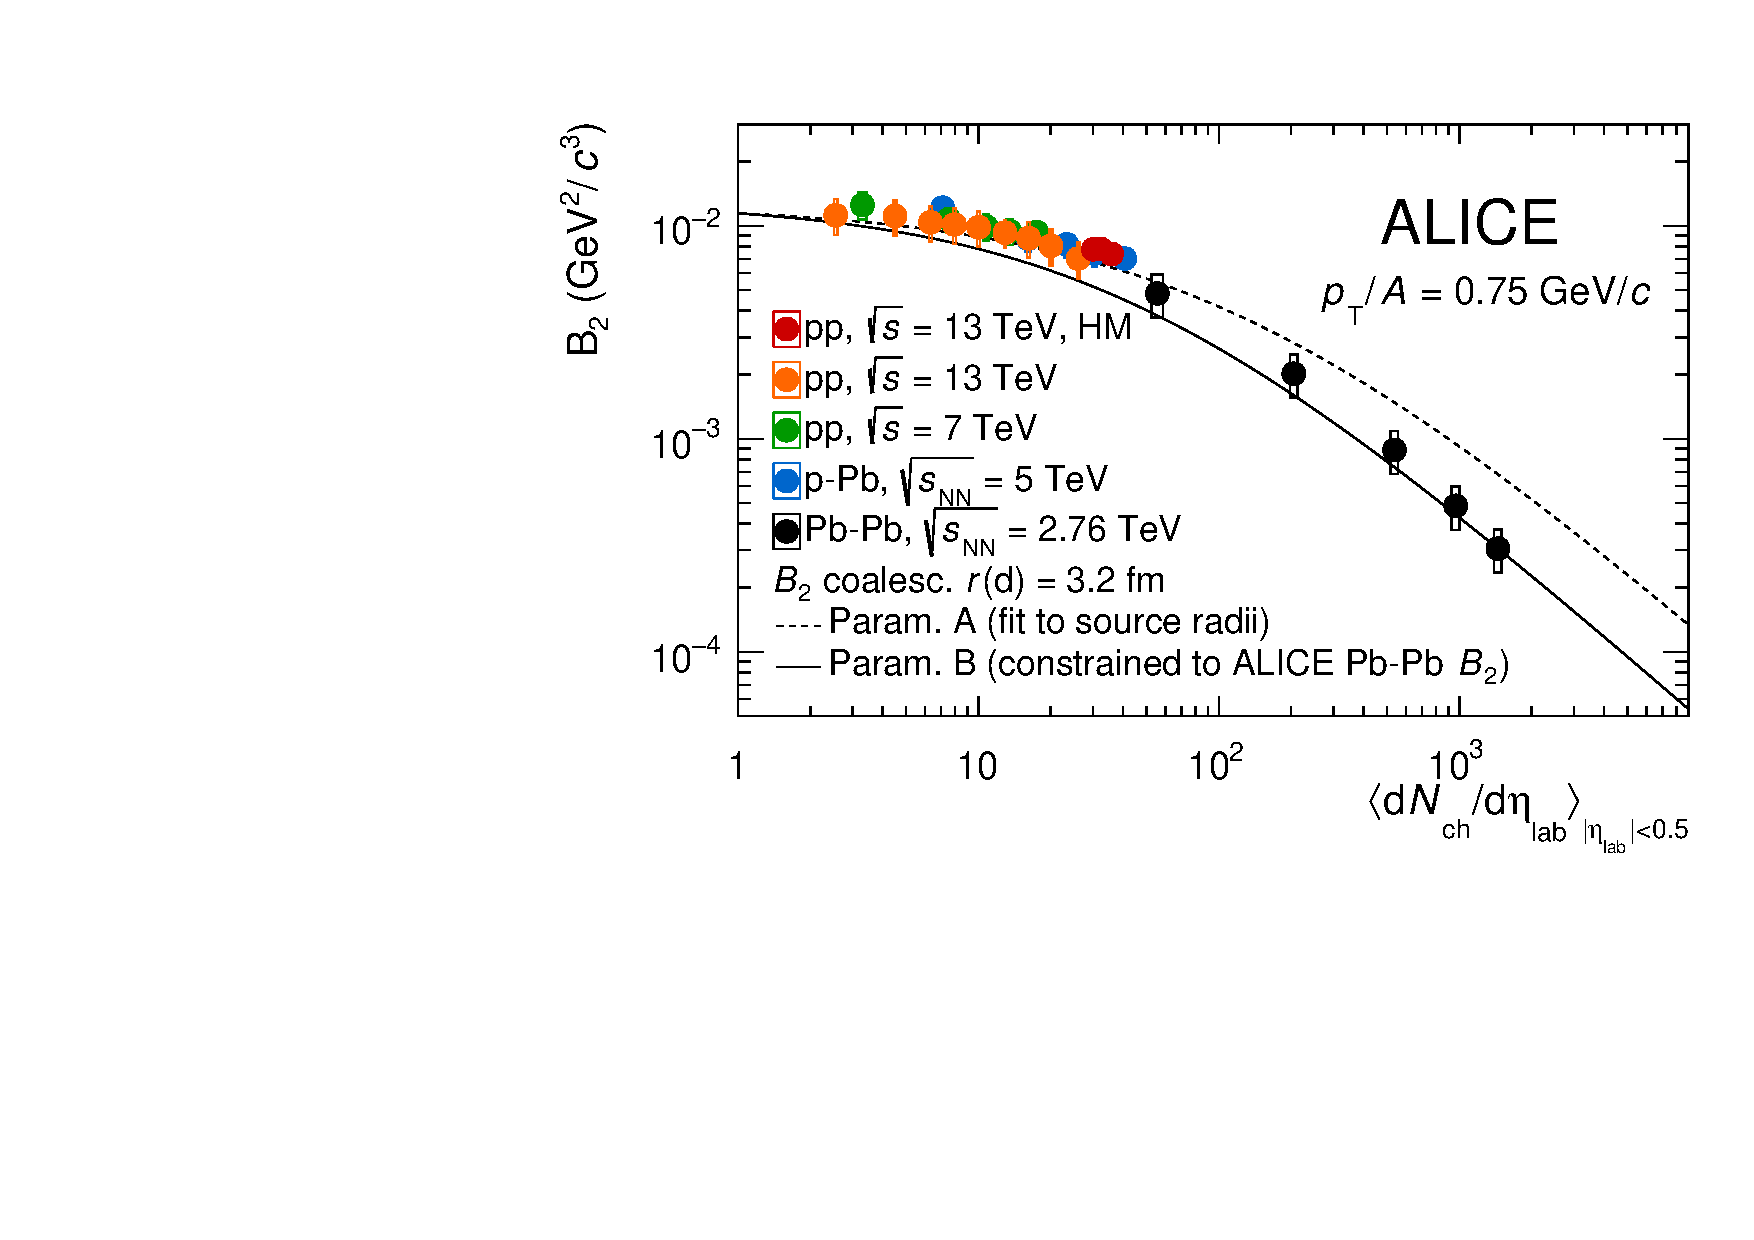
\includegraphics[width=\textwidth]{image/2-modelli/cB2vsMult.pdf}
        \caption{(Anti)deuteroni}
        \label{fig:cB2vsMult}
    \end{subfigure}
    %\hspace{1cm}
    \begin{subfigure}{.49\textwidth}
        \centering
        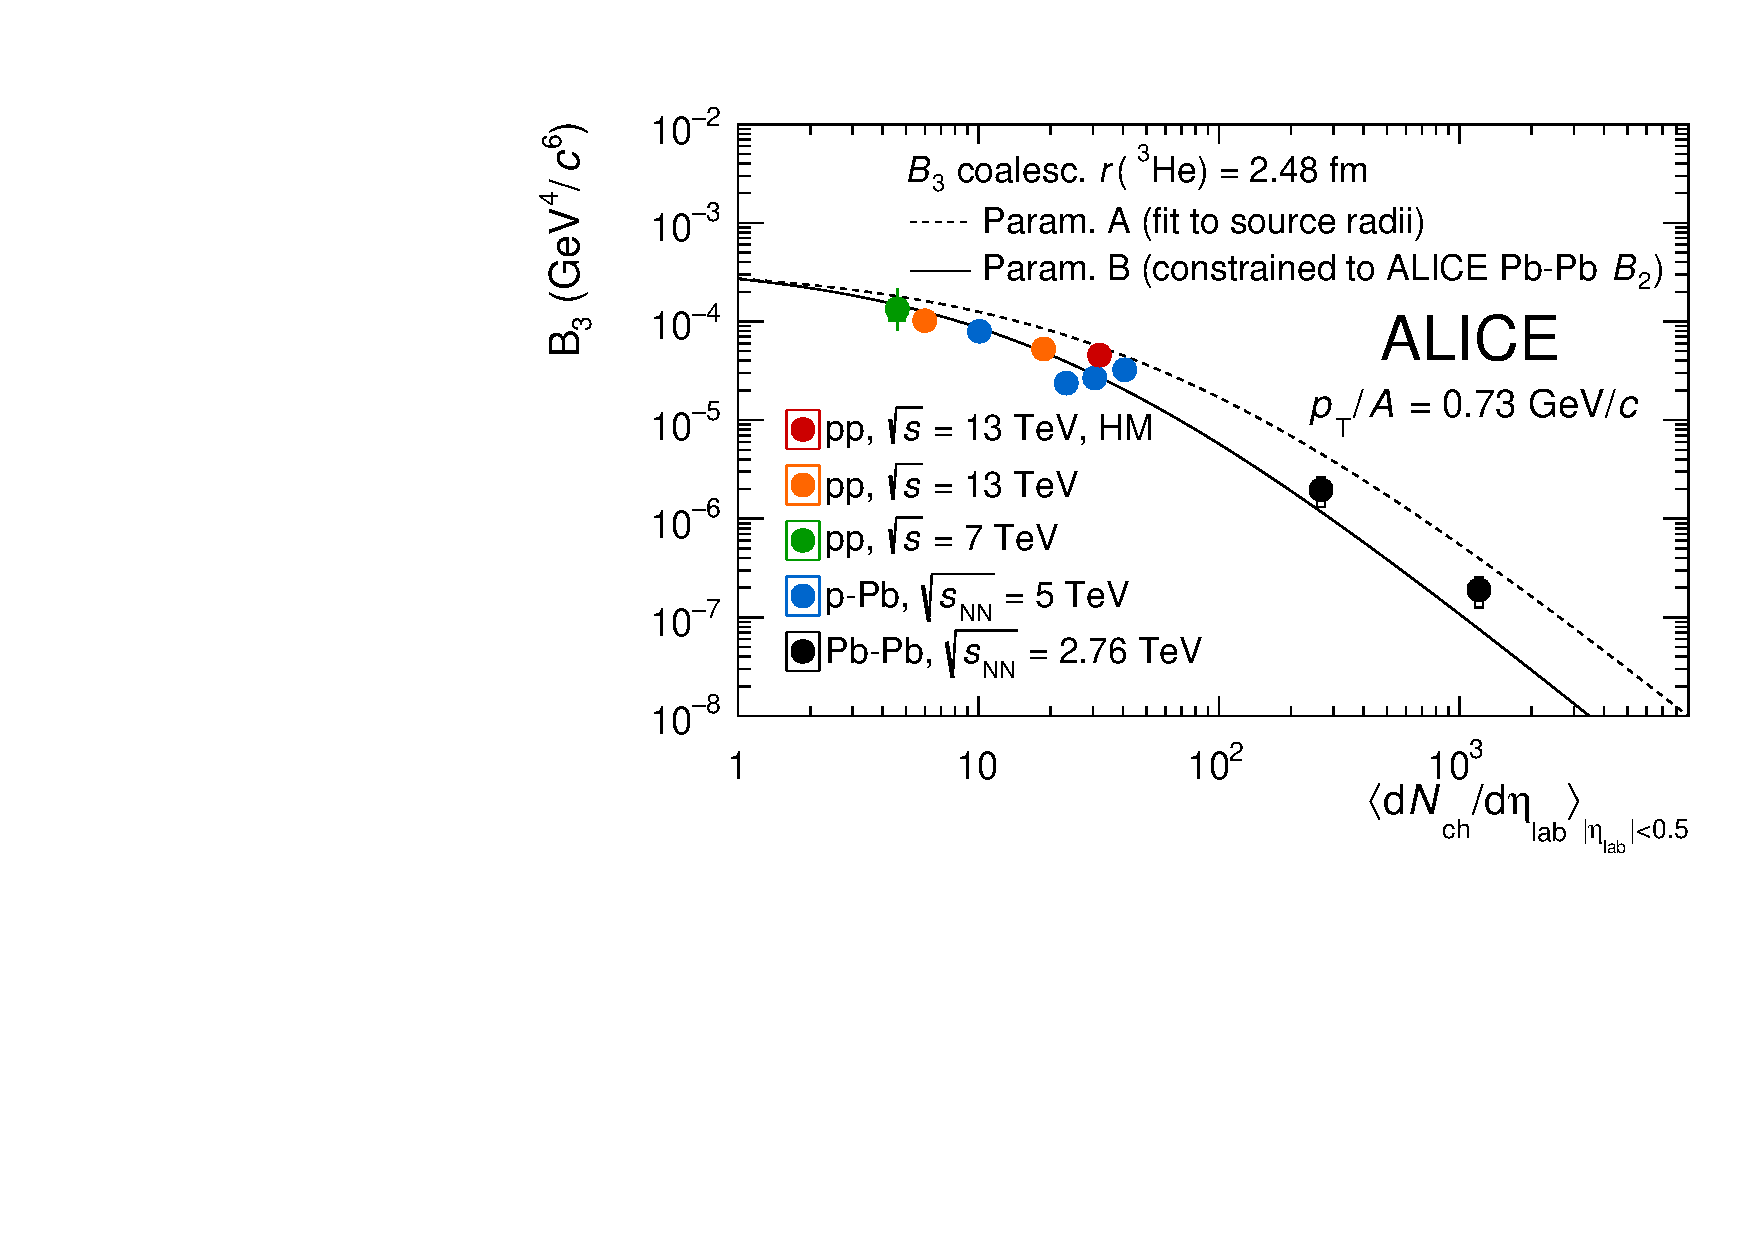
\includegraphics[width=\textwidth]{image/2-modelli/cB3vsMult.pdf}
        \caption{(Anti)elio}
        \label{fig:cB3vsMult}
    \end{subfigure}
    \captionwithsource{Misure (punti colorati) di \emph{\rmfamily (a)} $B_2$ e di \emph{\rmfamily (b)} $B_3$ in funzione della molteplicità effettuate a $p_t/A$ indicate. Le linee rappresentano le previsioni teoriche basate su due diversi parametrizzazioni del raggio della sorgente.}{\cite{alice_2022_coal_formula}} 
    \label{fig:BAvsMult}
\end{figure}
Si osserva che per la misura del parametro $B_2$, nelle collisioni a basse molteplicità (pp e p-Pb) $B_2$ ha una dipendenza debole della molteplicità, mentre per collisioni ad alta molteplicità (Pb-Pb) i dati mostrano un calo sostanziale di $B_2$. 
Analogamente per $B_3$, il modello di coalescenza descrive qualitativamente gli andamenti ma non riesce a farlo per tutto l'intervallo di molteplicità.